\chapterimage{head2.png} % Chapter heading image
\chapter{\normalsize Lecture notes: Diffusion Models}


\subsection*{1. Fundamental Concepts of Diffusion Models}

Diffusion models belong to the class of generative models --- models that describe a probability distribution $p$ and can generate samples from that distribution. They joined other generative approaches like Variational Autoencoders (VAEs), normalizing flows, and Generative Adversarial Networks (GANs).

Denoising Diffusion Probabilistic Models (DDPMs) were introduced in the paper by Ho et al.~[4]. Until their arrival, GANs were the dominant approach for high-quality image generation, despite being less probabilistically rigorous. DDPMs have since surpassed GANs in visual quality.

\subsection*{Key Differentiators from Other Generative Models}

In traditional generative models like VAEs and GANs, we learn to predict data (images) from latent vectors that follow a predefined distribution (often Gaussian). Diffusion models encode images differently --- by incrementally adding noise to the image over a pre-determined number ($T$) of time steps.

Two crucial differences from VAEs/GANs:
\begin{enumerate}
    \item \textbf{No dimension reduction} --- There is no inherent dimension reduction in the latent representations.
    \item \textbf{No semantic structure} --- The Step 0 latent representation contains no semantic or geometric information. Interpolating between two noised images will not generate semantically meaningful transformations.
\end{enumerate}

\section{The Forward Process (Diffusion/Noise Addition)}

The forward process is formalized as a Markov process $q$ that progressively adds noise to an image:
\begin{definition}[Forward Process of Diffusion Model]
\[
q(x_{1:T} \mid x_0) := \prod_{t=1}^{T} q(x_t \mid x_{t-1})
\]
where
\[
q(x_t \mid x_{t-1}) := \mathcal{N}(x_t; \sqrt{1 - \beta_t}x_{t-1}, \beta_t \mathbf{I})
\]
\end{definition}

Here, $\mathbf{I}$ is the identity covariance matrix over image space, and $\beta_t$ values are hyperparameters referred to as the variance schedule.

\subsection*{Closed-form Sampling}
A key insight is that we can derive a closed-form expression to directly sample a noisy image at any time step without having to sequentially add noise:
\begin{definition}[Closed form sampling]
\[
q(x_t \mid x_0) = \mathcal{N}(x_t; \sqrt{\bar{\alpha}_t} x_0, (1 - \bar{\alpha}_t)\mathbf{I})
\]
where $\alpha_t := 1 - \beta_t$ and $\bar{\alpha}_t := \prod_{s=1}^{t} \alpha_s$.
\end{definition}

\subsection*{Variance Scheduling}
For implementation, the original DDPM paper uses a linear variance schedule with $\beta_t$ increasing from $\beta_1 = 10^{-4}$ to $\beta_T = 0.02$. Alternative schedules like the cosine schedule have also been proposed, which emphasize later denoising steps.

\section{The Reverse Process (Denoising)}

The reverse process is where the main work happens --- the DDPM learns to generate noise-free images from their noisy representations. This iterative denoising is performed by a deep neural network that represents a joint distribution $p_\theta(x_{0:T})$.

\begin{definition}[Reverse Process (Denoising)]
Like the forward process, the reverse process is a Markov chain:
\[
p_\theta(x_{0:T}) := p(x_T) \prod_{t=1}^{T} p_\theta(x_{t-1} \mid x_t)
\]
where
\[
p_\theta(x_{t-1} \mid x_t) = \mathcal{N}(x_{t-1}; \mu_\theta(x_t, t), \Sigma_\theta(x_t, t))
\]

The process typically starts with an initial noise image $x_T$ drawn from a standard normal distribution:
\[
p(x_T) = \mathcal{N}(x_T; 0, \mathbf{I})
\]
\end{definition}

\section{Learning to Denoise}

Rather than predicting the denoised image $x_{t-1}$ directly from $x_t$, empirical research has found it easier to predict the noise $\epsilon$ that was used to generate $x_t$ from the original noise-free image $x_0$.

\subsection*{Reparameterized Forward Equation}
This uses the formula:
\begin{definition}[Reparametrization Trick]
\[
x_t = \sqrt{\bar{\alpha}_t} x_0 + \sqrt{1 - \bar{\alpha}_t} \, \epsilon
\]
The model is trained to predict $\epsilon_\theta(x_t, t)$, which estimates the noise $\epsilon$ from $x_t$.
\end{definition}

\subsection*{Architecture}
\begin{itemize}
    \item U-Net architecture is widely used as it's effective for image-to-image tasks
    \item Time point $t$ is included as an additional input
    \item At every down- and upsampling step, time is incorporated as a broadcast channel
    \item This broadcasted time representation is added to the image, similar to positional encoding
\end{itemize}

\subsection*{Loss Function}
The DDPM paper derives a Bayesian loss, but in practice a simpler MSE loss is used:
\begin{definition}[Loss Function]
\[
L_{\text{simple}}(\theta) := \mathbb{E}_{x_0, \epsilon, t} \left[\left\| \epsilon - \epsilon_\theta\left(\sqrt{\bar{\alpha}_t} x_0 + \sqrt{1 - \bar{\alpha}_t} \, \epsilon, t \right) \right\|^2 \right]
\]
\end{definition}
This is simply the mean squared error (MSE) between the predicted noise and the true noise $\epsilon$.

\section{Training and Sampling Process}


\subsection*{Training}
At each training iteration:
\begin{enumerate}
    \item Sample a random $x_0$ from data
    \item Sample a random time point $t$ uniformly from the $T$ time points
    \item Sample random noise $\epsilon \sim \mathcal{N}(0, \mathbf{I})$
    \item Compute the noisy image:
\begin{definition}[Noisy image at time $t$]    \[
    x_t = \sqrt{\bar{\alpha}_t} x_0 + \sqrt{1 - \bar{\alpha}_t} \, \epsilon
    \]\end{definition}
    \item Make a gradient update of the MSE loss w.r.t. $\theta$
\end{enumerate}
\begin{figure}[H]
    \centering
    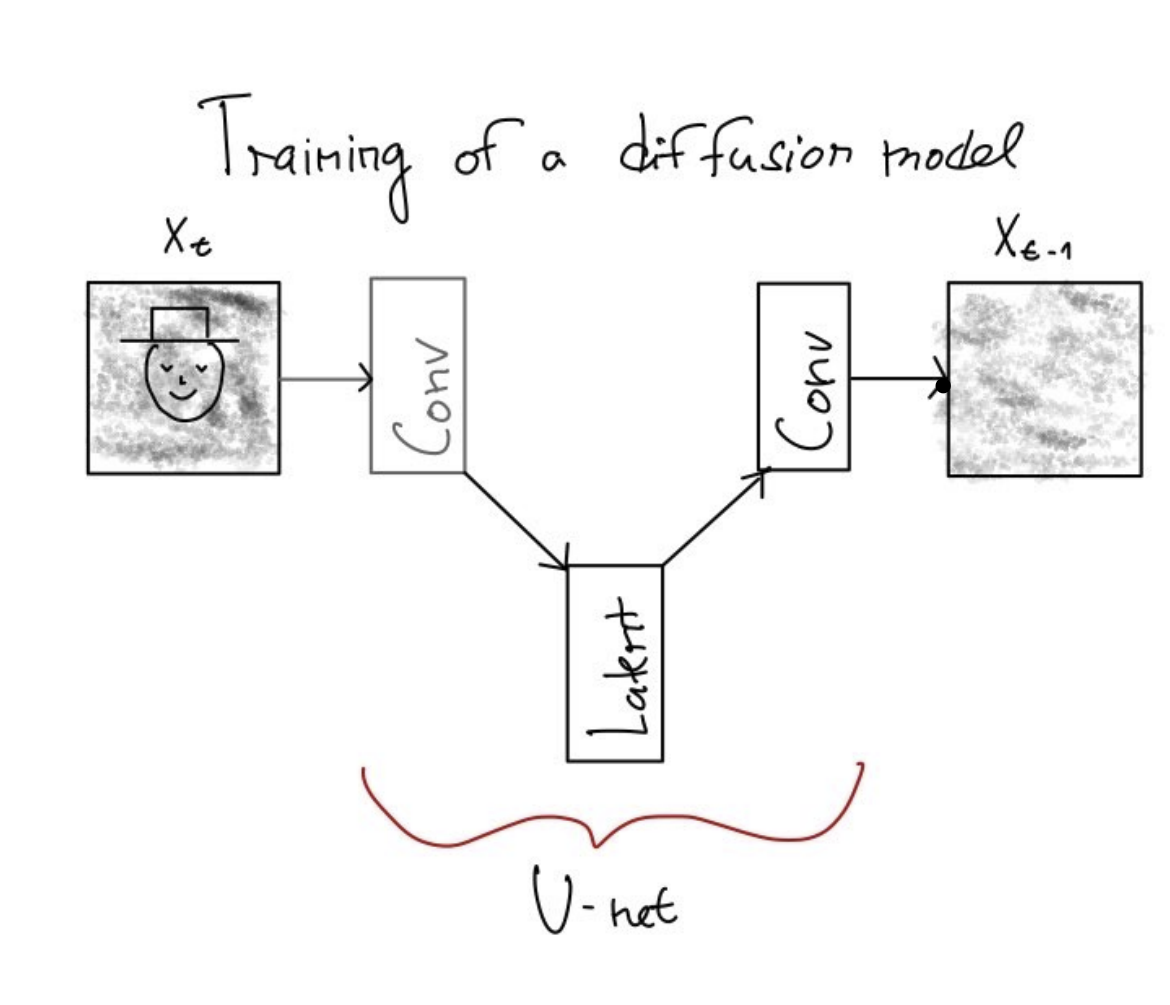
\includegraphics[width=1\linewidth]{billede.png}
    \caption{Illustration of the denoising diffusion process using a U-Net architecture. At each denoising step, the U-Net model $\epsilon_\theta$ predicts the noise component $\epsilon$ present in the noisy image $x_t$. Rather than directly predicting the clean image, the model outputs the estimated noise $\hat{\epsilon}_\theta(x_t, t)$, which is then subtracted from $x_t$ (with appropriate scaling based on the diffusion schedule) to obtain the less noisy image approximation $x_{t-1}$. This approach, where the network is trained to minimize $\mathbb{E}[\|\epsilon - \hat{\epsilon}_\theta(x_t, t)\|^2]$, has been shown to provide more stable training dynamics than directly predicting the denoised image.}
    \label{fig:unet_denoising}
\end{figure}
\subsection*{Sampling}
For sampling from the model:
\begin{enumerate}
    \item Set covariance $\Sigma_\theta(x_t, t) = \sigma_t^2 \mathbf{I}$, where $\sigma_t^2 = \beta_t$ (simplest version)
    \item Set mean:
    \begin{definition}[Denoising Mean Equation:]

    
    \[
    \mu_\theta(x_t, t) = \frac{1}{\sqrt{\alpha_t}} \left(x_t - \frac{\beta_t}{\sqrt{1 - \bar{\alpha}_t}} \epsilon_\theta(x_t, t)\right)
    \]
    \end{definition}
    \item Sample $x_{t-1} \sim \mathcal{N}(\mu_\theta, \Sigma_\theta)$
    \item Repeat iteratively to sample $x_{t-1}$ from $x_T$
\end{enumerate}



\section{Key Exam Topics and Common Questions}

\subsection*{What makes diffusion models different from VAEs and GANs?}
\begin{itemize}
    \item No dimension reduction in latent space
    \item Latent variables have no semantic structure
    \item Progressive noise addition/removal rather than direct encoding/decoding
    \item More stable training compared to GANs
    \item Better image quality than earlier models
\end{itemize}

\subsection*{What is the variance schedule $\beta_1 \ldots \beta_T$ and why is it important?}
\begin{itemize}
    \item Controls how quickly noise is added in the forward process
    \item Affects the difficulty of the denoising task
    \item Different schedules (linear, cosine) have different properties
    \item Cosine schedule focuses learning more on later denoising steps
\end{itemize}

\subsection*{Why do we predict noise $\epsilon$ rather than directly predicting $x_{t-1}$?}
\begin{itemize}
    \item Empirically proven to be easier and more effective
    \item Allows for a simpler loss function (MSE)
    \item Results in better performance
\end{itemize}

\subsection*{What architecture is typically used for diffusion models?}
\begin{itemize}
    \item U-Net architecture (originally designed for image segmentation)
    \item Modified to incorporate time as an additional input
    \item Time is broadcast as a channel and added at each scale
\end{itemize}

\subsection*{How is the sampling process defined in diffusion models?}
\begin{itemize}
    \item Start with pure noise $x_T \sim \mathcal{N}(0, \mathbf{I})$
    \item Iteratively denoise step by step using the learned model
    \item Each step involves sampling from a Gaussian with learned parameters
    \item Final result $x_0$ is the generated sample
\end{itemize}


\section{Practice Questions for Exam Preparation}

\begin{enumerate}
    \item \textbf{Q:} Explain the mathematical formulation of the forward process in diffusion models.\\
    \textbf{A:} The forward process is a Markov chain that progressively adds Gaussian noise to an image:
    \[
    q(x_{1:T} \mid x_0) := \prod_{t=1}^{T} q(x_t \mid x_{t-1})
    \quad \text{where} \quad q(x_t \mid x_{t-1}) := \mathcal{N}(x_t; \sqrt{1 - \beta_t} x_{t-1}, \beta_t \mathbf{I})
    \]
    This can be reparameterized to directly sample $x_t$ from $x_0$:
    \[
    q(x_t \mid x_0) = \mathcal{N}(x_t; \sqrt{\bar{\alpha}_t} x_0, (1 - \bar{\alpha}_t) \mathbf{I})
    \]

    \item \textbf{Q:} What is being learned by the neural network in a DDPM?\\
    \textbf{A:} The neural network is learning to predict the noise $\epsilon$ that was added to the original image, given a noisy image $x_t$ and time step $t$. This is then used to construct the parameters (mean and variance) of the reverse process distributions.

    \item \textbf{Q:} Why is the U-Net architecture suitable for diffusion models?\\
    \textbf{A:} The U-Net is designed for image-to-image tasks where spatial relationships matter. It has skip connections that help preserve spatial information. In diffusion models, we’re essentially doing image-to-image tasks: predicting noisy or denoised images with the same dimensions as the input.

    \item \textbf{Q:} How does the training objective differ from the theoretical formulation in the DDPM paper?\\
    \textbf{A:} While the theoretical loss is based on a variational lower bound, in practice a simpler MSE loss is used between the predicted noise and the actual noise. This was found to work better empirically.

    \item \textbf{Q:} What extensions to diffusion models might be covered in the next lecture?\\
    \textbf{A:} The next lecture will cover conditioning and guidance techniques, including classifier guidance, classifier-free guidance, universal guidance, and counterfactual explanations via diffusion models.
\end{enumerate}

\section{Common Pitfalls and Deep Insights}

\begin{itemize}
    \item \textbf{Latent Space Structure:} Unlike VAEs, the latent space in diffusion models lacks semantic structure, so traditional interpolation doesn’t work for tasks like “making a person smile.”

    \item \textbf{Computational Cost:} Diffusion models require sequential sampling through $T$ steps, making them slower than single-pass generators like GANs.

    \item \textbf{Theoretical vs. Practical:} There’s often a gap between theory and what works best in practice (e.g., simplified MSE loss performs better than variational losses).

    \item \textbf{Hyperparameter Sensitivity:} The variance schedule significantly affects performance and requires careful tuning.

    \item \textbf{Connection to Score-Based Models:} Diffusion models are closely related to score-based generative models – this insight may come up in deeper theoretical discussions.
\end{itemize}

\textbf{Reflection Prompt:} Be prepared to explain how you would approach the task of \textit{“making a person smile”} with a diffusion model, as this was posed as a discussion point in the notes.

